\chapter{Preliminary Work on Regression Analysis}
	\label{c:5}
The field of geo-distributed data analysis is quite vast. A detailed study of these aspects of the distributed approach of data analysis is beyond the scope of our tasks during the first few days. As a part of learning how to work on data analytic what we wanted to introduce is a problem specific approach. We were interested in doing ``Regression Analysis" on data located at different geographical areas all around the world. Primarily we have worked out with only two variants of regression analysis ``Linear Regression" and ``Polynomial Regression". So we can say the other variants as well as other problem oriented approaches were not be covered in this chapter. 

\section{Contribution}
Summarizing, our main contributions are:
\begin{itemize}
\item We propose an approach of regression analysis that is deals with geo-distributed data and provide an in-depth study of the relative merits against centralized approach.
\item We propose a system that builds upon Apache Hadoop MapReduce \cite{116} framework and extends their functionality to support multi data center learning applications.
\item We propose an approach that will minimize the number of transfers among data centers thus minimize the inter data center bandwidth utilization.
\item We propose an approach that is a combination of the two concepts \emph{Data Parallelism} \cite{117} and \emph{Model Parallelism} \cite{117}.
\item We present experimental results implemented on \emph{Amazon Web Services (AWS)}. 
\end{itemize}

\section{Problem Specification}
We were interested in building a regression model on geographically distributed data. We had the intention of using least square regression analysis. In order to facilitate the study, we formalize the problem in two dimensions: 
\begin{enumerate}
\item We will make our assumptions about the data, its type, size and distribution.
\item We limit the regression analysis to 2nd order only. That means we would try only ``Linear Regression" and ``Polynomial Regression".
\end{enumerate}
So we can see that regression analysis on higher order and other classes of regressions (eg. ``Logistic Regression") will not be covered in this paper.

\subsection{Assumptions on Data}
To keep the analysis simple we used data only in text format. There may be multiple text files which will be considered as input files to our program. every text file contains multiple lines and each of these lines will be tokenized and the information will be extracted.

\subsection{Distribution of Data}
In order to run our program on distributed data we used cloud computing facilities of \emph{Amazon Web Services (AWS)}. We created two different data centers in two different geographic location, ``North Virginia" and ``Malaysia". Every data center was consisted of two \emph{Linux} instances. Among the two instances  of a data center we named one of  them as \emph{NameNode} and other one as \emph{DataNode}. The \emph{NameNode} works as a master node of its corresponding data center. Full data of a particular data center is further distributed in its \emph{NameNode} and \emph{DataNode}. Any kind of jobs on the the data of a data center can also be split and distributed among its instances. 


\section{Approach}
We created \emph{Hadoop MapReduce} cluster on \emph{Amazon AWS}. Our implementation needs to obtain resources like CPU cores, Memory during the partial computation on data in a particular data center in a uniform basis. Such resources are managed by a resource manager in the \emph{Hadoop} cluster system. Further, \emph{Apache Hadoop YARN}'s new federation feature allows us to view multiple data centers as a single one.
Data on a data center is organized by \emph{Haddop} File System \emph{HDFS}. 

\subsection{Learning Process}
For running our regression computation on geographically distributed data we mainly focused on two concepts:
\begin{itemize}
\item \textbf{Data Parallelism} It is the main idea of distributed data. Its can be seen as application of a single instruction to multiple data items. It focuses on distributing the data across different nodes, which operate on the data in parallel. As an example we can mention the array operations. In case of summing the data of an array, we can make multiple partition of the array and then apply summation formula on each partition. The aggregated result will give us the final summation. In our distributed data organization, data are located in different location while we need to make the same computation on them. This can be achieved by making partial computation on each data partition and aggregate them at the end.   

\item \textbf{Model Parallelism} In case of model parallelism the system gives every processor the same data but applies a different model to it. Model parallelism finds its applications in deep learning. As we can see that data centers are generally composed of multiple machines, we can use that resource to speed up the computation. If any learning process consists of multiple types of computation then we can create different model and place them in different machines. Therefore, at the time of making partial learning from any data center, each machine can do its model task on a parallel basis and the whole result can be obtained at a lower time period.
\end{itemize}

The first innovation in our approach is that we intend to make a mixed use of both \emph{Data Parallelism} and \emph{Model Parallelism}. 
\begin{itemize}
\item Data that are distributed in different data centers located at different geographic location resemble the \emph{Data Parallelism} concept. 
\item Then in case of a single data center, every machines of that data center has a shared view on the data because of the \emph{HDFS} file system. In order to compute $n$ parameters, if the data center has $n$ machines then we can distribute the different computation in different machines. That means every machine will work on separate models in parallel. This gives the use of model parallelism. 
\end{itemize}


The parameter to passed among the data centers can be determined from the equations or regression. For example of we consider regression of second degree, it can be expressed as:
\begin{align*}
y &= y_{model} + \epsilon\\
y_{model} &= ax^2 + bx + c
\end{align*}
where,
\begin{align*}
y &= original\ value\\
y_{model} &= model\ value\\
\epsilon &= error\\
\epsilon &= y - y_{model}\\
\end{align*}




If we intend to use least square regression model then we have to minimize the total squared error


\begin{align*}
S &= \sum \epsilon ^ 2\\
&= \sum (y-y_{model})^2
\end{align*}

In the process of minimizing $S$ we get the necessary equation to find the co-efficients in matrix form:

\[
\left[
\begin{array}{ccc}
\sum x_i^4 &\sum x_i^3 &\sum x_i^2 \\
\sum x_i^3 &\sum x_i^2 &\sum x_i \\
\sum x_i^2 &\sum x_i &n
\end{array}
\right]
\left[
\begin{array}{c}
a\\b\\c
\end{array}
\right]
=
\left[
\begin{array}{c}
\sum x_i^2y\\\sum x_iy_i\\\sum y_i
\end{array}
\right]
\]

Here we have to compute 7 parameters that appear in the matrix form. Every data center will compute these parameters on its own data. Then they will be sent to the initiating data center. At the initiating data center all the parameter will be merged to get the final model.

\subsection{Algorithm}
The whole process is divided into two parts. First of all, every data center will compute parameters by executing computation on their corresponding partial data. This task will be handled by the child processes. And the initiating data center i.e. master data center will run the parent process. which will receive the partial computational result and merge them to built a complete regression model.

\begin{algorithm}[!htbp]
	\caption{Geo-Distributed Regression Analysis}
	 \label{algo:1}
	\begin{algorithmic} [1]
	\STATE \textbf{Input: }Data located at different geographic location
	\STATE \textbf{Output: }Regression model
	\STATE \underline{Parent Process}
	\STATE select an arbitrary data center as the initiating one, \emph{root}
	\WHILE{end of ``node list'' has not encountered}
		\STATE pick a data center, \emph{node}
		\STATE create a parallel executable child process with the parameters \emph{root} and \emph{node}
	\ENDWHILE
	\STATE $available = false$
	\WHILE{$available = false$}
		\IF{every partial computational files from every data centers are available}
			\STATE $available = true$
		\ENDIF
	\ENDWHILE
	\STATE merge all the partial computational files into a single one
	\STATE create final regression model using the merged files
	\end{algorithmic}
\end{algorithm}



\begin{algorithm}[!htbp]
    \caption{Geo-Distributed Regression Analysis}
	\begin{algorithmic} [1]
	\label{algo:2}
	\STATE \textbf{Input: }{Data located in corresponding local machines}
	\STATE \textbf{Input: }{Information of 2 nodes}
    \STATE \textbf{Output: }{Partial Parameter}
	\STATE \underline{Child Process}
	\STATE set the input and output locations of \emph{Hadoop} File System
	\STATE run the “Partial Regression Computation” program
	\IF{root and node are the same}
	
		\STATE the $node$ is the initiating data center $root$ itself
		\STATE rename the output files with information of $root$
		\STATE move the renamed files in the $Common Container$ location of $root$
	
	
	\ELSE
	
		\STATE the $node$ is a non initiating data center
		\STATE rename the output files with information of $node$
		\STATE send the renamed files in the $Common Container$ location of $root$
	
	\ENDIF
	\end{algorithmic}
\end{algorithm}


\newpage

From the algorithm, we can see that there will be two types of communication during the learning task:
\begin{itemize}
\item \textbf{Global Communication}
Every data center has multiple instances of machines. Among them only one will communicate with other data centers. Such machine will be considered as a master node. There will be message passing among the master nodes of data centers. Whenever a learning process is to be initialized one of the master nodes will issue command to each master nodes to start their partial computation. Again after the partial computation of each data centers the parameters will be passed towards the initializing data center's master node. In this way the master nodes of every data center will create a Global Communication Group among them.
\item \textbf{Local Communication}
Whenever a data center's master node receives the command of partial computation, it will communicate with its other machines i.e. slave nodes. The computation task will be distributed among all the machines of that data center in order to exploit the advantage of \emph{Model Parallelism}. We can say that each machine of a data center will work on one or some specific job. At the completion of each job each separate machine will write its result in a common container of the master node from where all the partial results will be transferred to initialing data center's master node.
\end{itemize}
The communication group are shown in Figure \ref{communication}


\begin{figure}[!htbp]
\centering
\frame{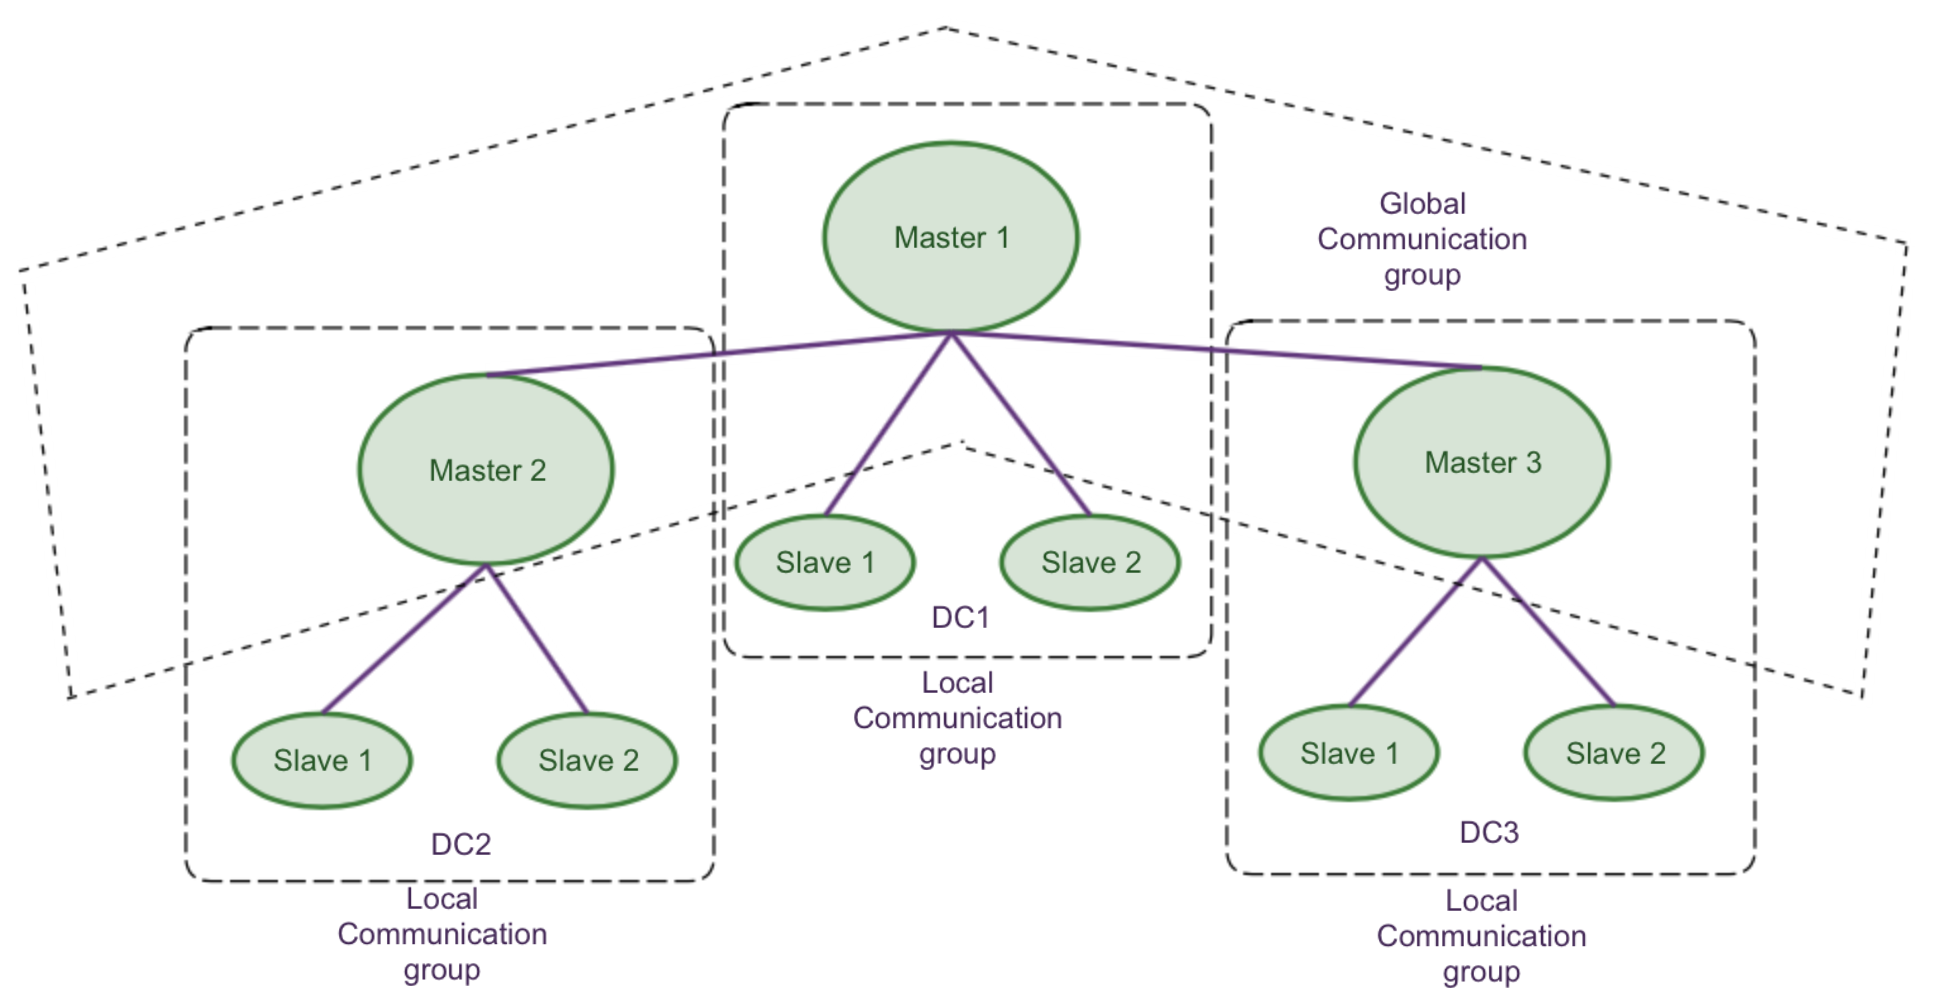
\includegraphics[width=5.2in]{communication.png}}
\caption{Communication Groups}
\label{communication}
\end{figure}


Figure \ref{learning} shows how the algorithms works. Here direction of the arrows shows the transfer direction.

\begin{figure}[!htbp]
\centering
\frame{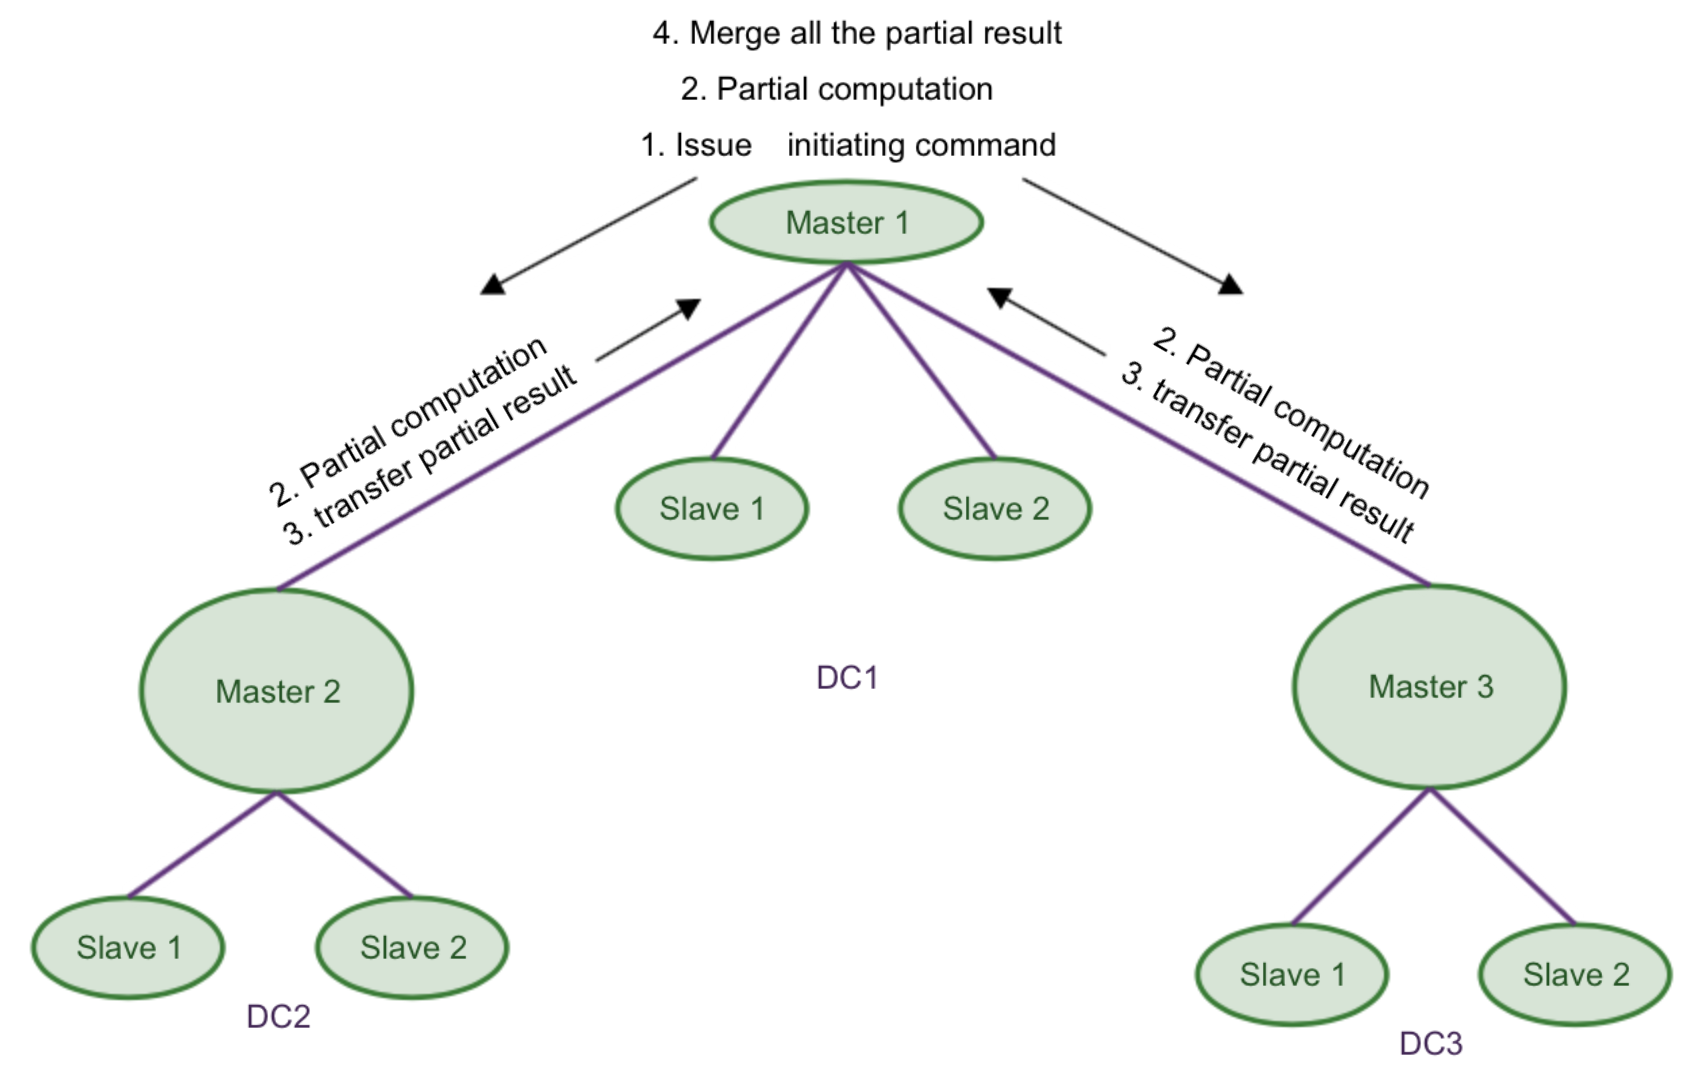
\includegraphics[width=5.2in]{learning.png}}
\caption{Graphical Interpretation of Learning Algorithm }
\label{learning}
\end{figure}

\newpage

\section{Our Implementation}
For the main program we used \emph{Hadoop MapReduce} framework. We used \emph{Java} as programming language. For inter data center communication we used \emph{Secure Shell (SSH)} Protocol. For some extra works we had to use \emph{C++} programming language also. 
\subsection{How the Distributed Algorithm Works}
A shell script initializes the whole learning process. Master node of every data center will contain this program file. Every data center will have the information of other data centers where data reside in distributed fashion. This program will read every other data center's information and with this information it will start another child program along with it's own information.

The child program receives information of all the data centers one by one. Then it will communicate with that data center and issue a command  to start it's internal computation for parameters to build a complete regression model.

The child process will match the information of two data centers passed to it. If it is the initiating data center, then it will start some master task. Other wise slave tasks will be initiated.

At first environment variables associated with \emph{Hadoop MapReduce} will be set up. At this point the main program of computing partial results will be executed on every data centers. The program is based on mapping input data into specific intermediate outputs and then reducing them. For example, while running the computation model of $\sum x^k$, the map function will map every $x$ into $x^k$ and send to the reducer. The corresponding reducer will sum all those   $x^k$ to generate $\sum x^k$. 

When the partial computational output is available in initiating data center, this program will rename the output files with appropriate names including corresponding data center information and move them into a common container. 

The main difference of non initiating data centers is rather than moving the renamed files this program will send those files to the common container. 

When all the partial computations are completed, the margin process will combine all the files of this container. 


\subsection{Runtime Analysis}
If the size of data is $n$, i.e. there are $n$ rows in every sample input then in the \emph{MapReduce} program, the number of maps for each parameter model will be $O(n)$. If the number of parameters to be generated is $p$ and number of machines is $\frac{p}{m}$ then the number of maps will be $O(mn)$\\
If the reducer of a parameter merges every two intermediate outputs of corresponding mapper then we can minimize the number of reducers to $O(\log _2 n)$. Therefore if the number of machines  is $\frac{p}{m}$, the number of reducers will be $O(m\log _2 n)$..

\section{Experimental Findings}
In case of finding any parameter, while any job is submitted it takes few time or its initial setup. For analyzing the result we ignored that  setup time by finding it empirically.
First of all we show the time vs data size graph. From Figure \ref{time vs size}, we can see that the time grows almost linearly with the size of data. 



\begin{figure}[!htbp]
\centering
\frame{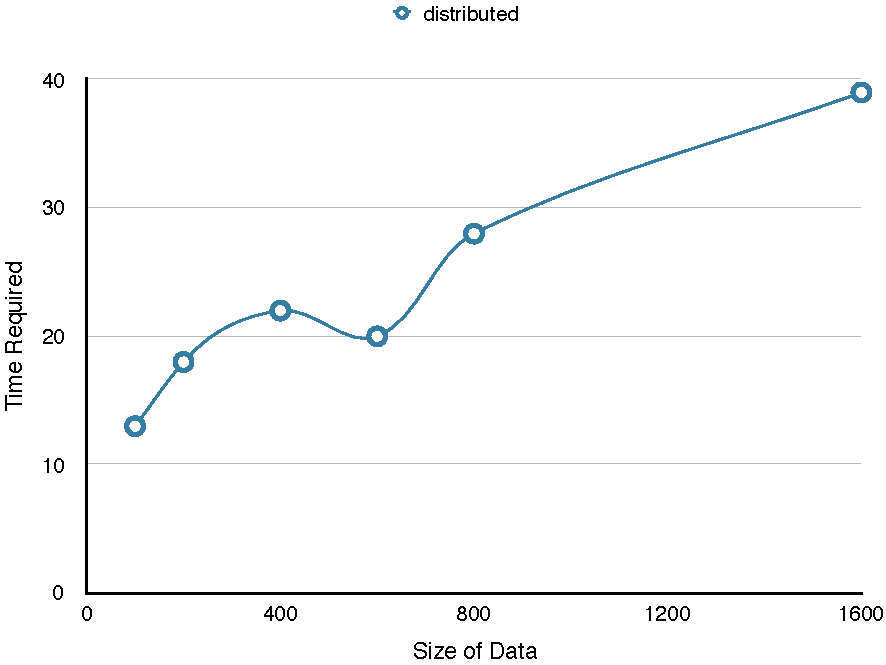
\includegraphics[width=5.2in]{dist.pdf}}
\caption{Time Required vs Data Size graph of our Distributed Approach}
\label{time vs size}
\end{figure}


A comparison between centralized approach and our distributed approach is shown in Figure \ref{cent vs dist}. We can easily see that time required for centralized approach is growing at a pretty high rate than that of the distributed approach.



\begin{figure}[!htbp]
\centering
\frame{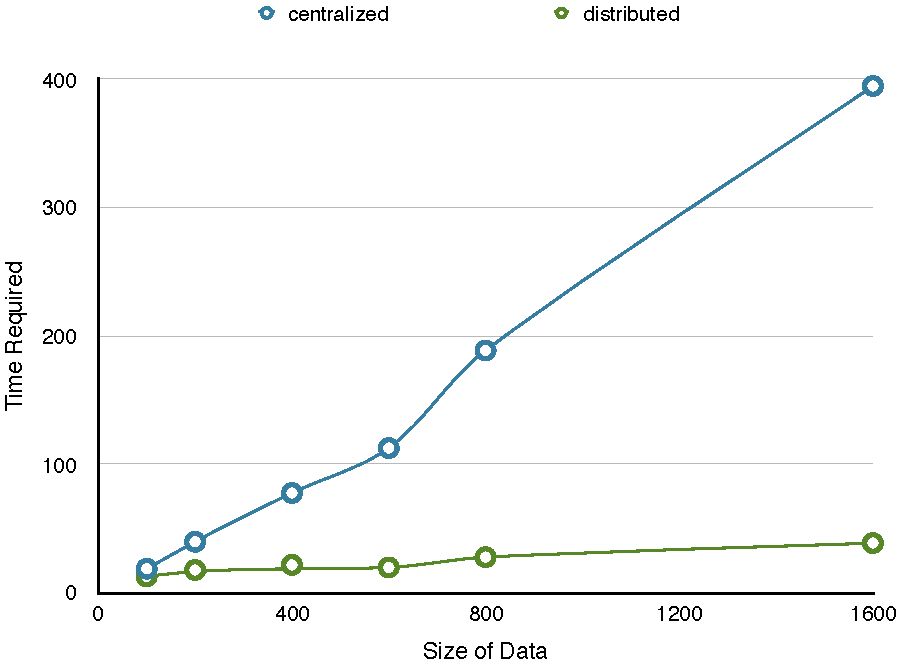
\includegraphics[width=5.2in]{centvsdist.pdf}}
\caption{Comparison graph between centralized and distributed approach}
\label{cent vs dist}
\end{figure}



As we were making an use of \emph{Model Parallelism}, the number of instances in a data center plays a big role in the computational runtime. We can demonstrate it by an example. 
\begin{itemize}
\item In case we have $n$ models to run and have $\frac{n}{k}$ instances in a data center. Then every instance will be assigned to run $k$ models. It means these $k$ models will run at a sequential basis. Obviously the number $k$ is preferable to be as low as possible.
\item The best result can be found with $k=1$. While the number of instances are equal to the number of models then every model can be run in parallel. Then the total runtime will be the  time  of the worst time taken model.  
\end{itemize}

As we were using free tires of $750$ hours in \emph{Amazon Web Services}, we did not have the scope to use as more instances as possible. In fact, we could  only use 3 instances at most for every data center. Still it showed a significant variance in runtime while running on different number of instances. In Figure   
\ref{instances}, we can see that the run time decreases as the number of instances increases.

\begin{figure}[!htbp]
\centering
\frame{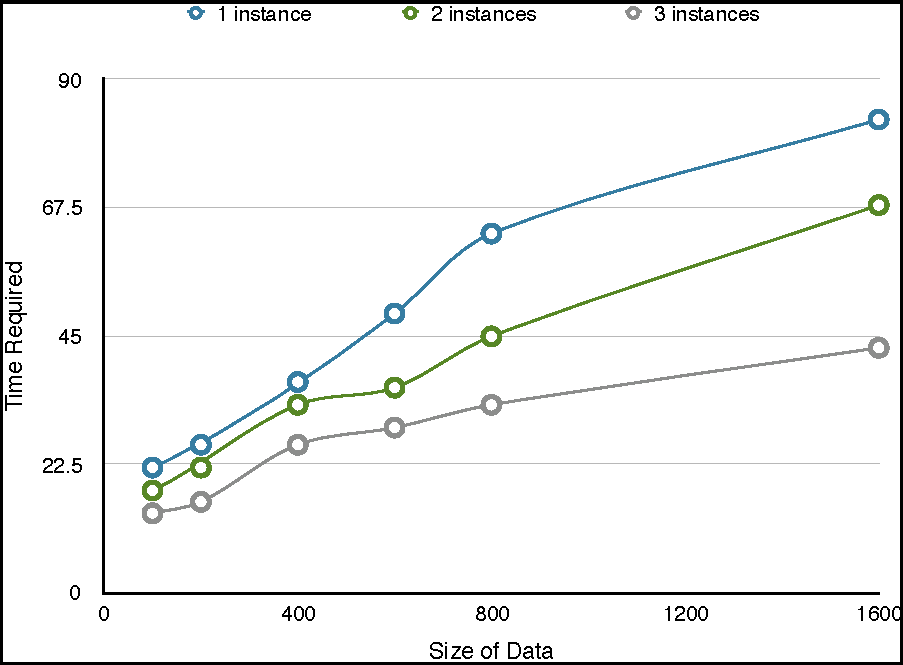
\includegraphics[width=5.2in]{instances.pdf}}
\caption{Comparison graph based on number of instances}
\label{instances}
\end{figure}



\newpage
\section{Limitations}
We used a general approach to create the regression models for both linear and polynomial regression. Each data center does its portion of computation on its own data. We applied the approach on mainly text input files where each file consisted of multi line texts. For each line we extracted 2 parameter as $x$ and $y$. Here we can see that we are finding sums such that $\sum x^2$, $\sum x^3$, $\sum y^2$, $\sum y^3$ etc. To be specific in order to create a linear regression model we need to calculate sums of exponents of $x$ and it was up to $\sum x^2$ then for polynomial it was up to $\sum x^4$. In general it can be observed that for a regression analysis of $n$th order we need to calculate up to $\sum x^{2n}$ and have to send $3n+2$ numbers of such summation values to a central data center. So we can see that using higher order regression analysis it will become practically impossible to use this approach. 

More problems arise while $x$'s carry large values. In case of polynomial regression if in general every data center has one billion $10^9$ line text input in data files and the average value of $x$ is in range $10^3$, then the system will have to handle sum values in the range of $10^{21}$. A different approach of handling such big numbers should be followed to make the approach more useful.   

The time required for the computations of parameters are not same. Primarily, in case of using \emph{Model Parallelism} if we have exactly same number of instances and models then we assume to have the best runtime. But all the models dont take the same time. As a result the load of running models can be further distributed among idle instances. Whenever any low time consuming model is finished in any instance, it becomes idle and any high time consuming model can be split and a portion can be assign to run in such idle instances.

\endinput